\chapter{Pico Subsystem}\label{ch:sw-pico-sys}

\begin{figure}[htbp]
    \centering
    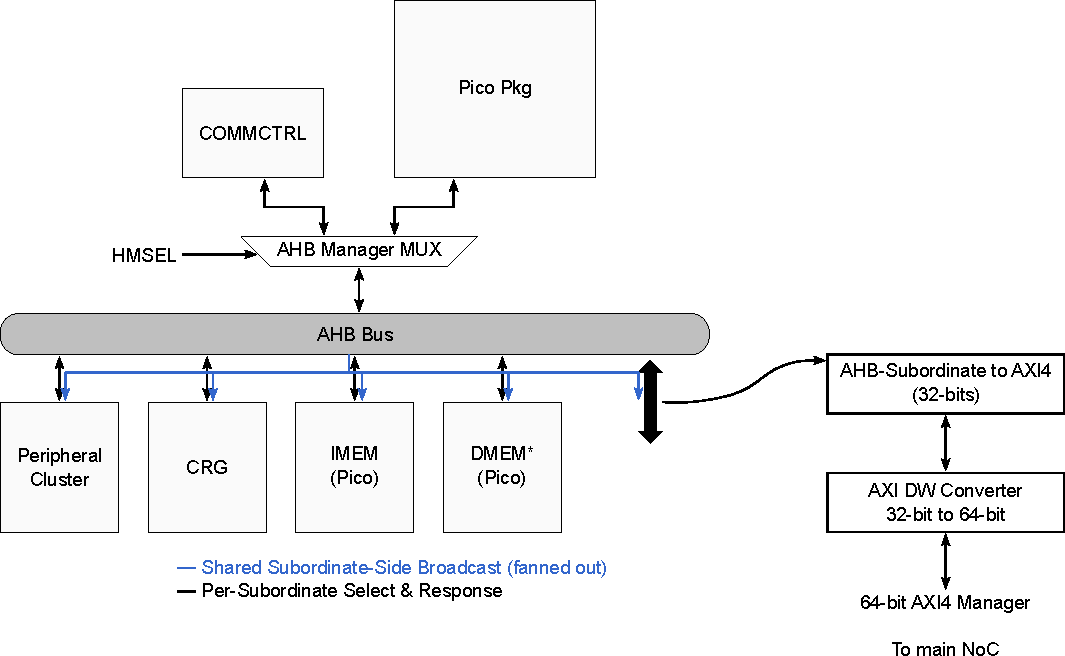
\includegraphics[width=0.95\textwidth]{figures/pico_subsys_blk.pdf}
    \caption{Pico subsystem block view.}
    \label{fig:picosys-blk}
\end{figure}

The Pico subsystem is the SoC's control plane. It couples the PicoRV32 core (as \hyperref[sec:sw-pico-pkg]{Pico Package}) with the host command interface, \hyperref[sec:sw-commctrl]{COMMCTRL}, the on-chip control registers (\hyperref[sec:sw-crg]{CRG}), and the Pico-local peripherals (\hyperref[sec:sw-peripheral-cluster]{Peripheral Cluster}), all joined by an \hyperref[sec:sw-ahb-bus]{AHB Bus}. It is the first block to wake at power-on and is responsible for loading and releasing the Rocket core (\autoref{ch:sw-rocket-sys}). See Figure~\ref{fig:picosys-blk}. 

\section{Pico Package}\label{sec:sw-pico-pkg}

PicoRV32 core is a lightweight, auxilary core developed by Yosys. It implements RV32IMC instruction set. More generally, it can be configured as an RV32E, RV32I, RV32IC, RV32IM, RV32IMC core. It has the following features\footnote{PPA results reproduced here from the repository without any additional verification.}:
\begin{itemize}
  \item Small, lightweight core requiring about 750 -- 2000 LUTs in 7-Series Xilinx Architecture. 
  \item High \(f_\mathrm{max}\) of about 250 -- 450 MHz on Xilinx FPGAs. 
  \item Three options for interfaces: Native Memory (\texttt{picorv32}), AXI4-Lite Manager (\texttt{picorv32\_axi}), or Wishbone (\texttt{picorv32\_wb}).
  \item A built-in interrupt controller with optional, custom ISA support.
  \item An optional co-processor interface. 
  \item Configurable RF: It is possible to disable support for the registers \texttt{x16 - x32}, as well as \texttt{RDCYCLE[H]}, \texttt{RDTIME[H]}, and \texttt{RDINSTRET[H]} instructions\footnote{Refer to the official RV32E ISA.}. The RF can be configured as single or dual ported. 
\end{itemize}

\textbf{Relevant Link(s):} \begin{itemize}
  \item \href{https://github.com/YosysHQ/picorv32}{PicoRV32 Repository}
  \item \href{https://github.com/whatmough/CHIPKIT.git}{COMMCTRL/CHIPKIT Repository}
  \item \href{https://github.com/adki/gen_amba_2021.git}{AMBA Bus Generator Repository}
\end{itemize}

The \texttt{pico\_pkg\_ahb} bridges the native-memory PicoRV32 core to the subsystem as a single AHB-Lite manager. The package attaches the core's private on-chip SRAM memory and fixes the boot
convention:
\begin{center}
  \begin{tabular}{c c}
    \toprule
    \textbf{Region} & \textbf{Base} \\
    \midrule
    .global, .text, .rodata, .data & \texttt{0x0000.0000}\\
    Stack & \\
    \bottomrule
  \end{tabular}
\end{center}

The reset vector is \texttt{0x0000.0000}, and the initial stack pointer\todo{FIX THIS RATIO!} is placed at the top of the print-buffer region (\texttt{0x0001.FC00}). The host loads Pico firmware into IMEM through COMMCTRL before handover.

\section{COMMCTRL}\label{sec:sw-commctrl}

The COMMCTRL is a UART-based communication controller. It is capable of accessing i.e., reading and writing to any address in the 32-bit address space\footnote{The address should have meaning of course, else it might cause an illegal access trap somewhere in the SoC or return a garbage value.}. To use this module, UART interface is exposed over which binary form of the ASCII representation of the read and/or write commands is stream. 

The format of a write command is as follows:
\begin{center}
    \begin{tabular}{c c}
        \toprule 
        Byte & Field \\
        \midrule
        0 & ASCII (W or w)\\
        1 & single whitespace \\
        2 & 0 \\
        3 & ASCII(X or x)\\
        4 - 11 & WRADDR \\
        12 & single whitespace \\
        13 & 0 \\
        14 & ASCII(X/x) \\
        15 - 22 & WRDATA \\
        23 & CR \\
        24 & LF \\
        \bottomrule
    \end{tabular}
\end{center}
and a read command is formatted as:
\begin{center}
    \begin{tabular}{c c}
        \toprule 
        Byte & Field \\
        \midrule
        0 & ASCII (R or r)\\
        1 & single whitespace \\
        2 & 0 \\
        3 & ASCII(X or x)\\
        4 - 11 & RDADDR \\
        12 & CR \\
        13 & LF \\
        \bottomrule
    \end{tabular}
\end{center}
While the write command is 25 bytes large, the read command is shorter and is zero-padded to match this length. As shown in Figure~\ref{fig:picosys-blk}, the COMMCTRL and Pico package are multiplexed as managers of the AHB-Lite bus. The control of this AHB MUX is handled by writing to the location 0x1000.0000. Particularly, writing a 1 to this location using the COMMCTRL hands over the control to the Pico package. Writing a 0 relinquishes the control back to the COMMCTRL. 

Because it is a bus master, the host can load the Pico IMEM, load the Rocket memories across the NoC, and
read results back. 
\begin{center}
  \begin{tabular}{@{}lll@{}}
  \toprule
  \textbf{Address} & \textbf{Symbol} & \textbf{Effect} \\
  \midrule
  \texttt{0x1000\_0000} & \texttt{COMMCTRL\_HANDOVER\_ADDR} & Host writes 1 to hand bus ownership to the Pico. \\
  \texttt{0x1000\_0004} & \texttt{COMMCTRL\_IRQ\_ADDR}      & Host write raises a one-cycle COMMCTRL interrupt. \\
  \bottomrule
  \end{tabular}
\end{center}


\section{AHB Manager MUX and Bus}\label{sec:sw-ahb-bus}
The \texttt{pico\_ahb\_bus} is the subsystem interconnect. It arbitrates two managers, COMMCTRL and the Pico core, onto one AHB fabric and decodes the address to select a subordinate. Ownership is
explicit: at power-on COMMCTRL holds the bus and loads memory; when the host writes the handover address (\autoref{sec:sw-commctrl}), ownership passes to the Pico core, which then runs its firmware. Addresses that do not fall in a local subordinate are forwarded to the NoC through the AHB-to-AXI bridge (\autoref{ch:hw-pico-sys}). 

The address space \texttt{0x0000.0000 - 0x2000.0000} is reserved for the managers of the PicoSys and includes the on-chip SRAM memory of the Pico core, the control registers defined by CRG, and the peripheral cluster.   

\section{Clock and Reset Generator (CRG)}\label{sec:sw-crg}

\section{Peripheral Cluster}\label{sec:sw-peripheral-cluster}